\documentclass[a4paper,11pt,titlepage]{report}
\usepackage[printonlyused]{acronym}
\usepackage{amsmath}
\usepackage[UKenglish]{babel}
\usepackage{caption}
\usepackage{color}
\usepackage[hidelinks]{hyperref}
\usepackage{graphicx}
\usepackage[T1]{fontenc}
\usepackage[utf8]{inputenc}
\usepackage{listings}
\usepackage{lmodern}
\usepackage{url}
\renewcommand{\texttt}[1]{%
  \begingroup
  \ttfamily
  \begingroup\lccode`~=`/\lowercase{\endgroup\def~}{/\discretionary{}{}{}}%
  \begingroup\lccode`~=`[\lowercase{\endgroup\def~}{[\discretionary{}{}{}}%
  \begingroup\lccode`~=`.\lowercase{\endgroup\def~}{.\discretionary{}{}{}}%
  \catcode`/=\active\catcode`[=\active\catcode`.=\active
  \scantokens{#1\noexpand}%
  \endgroup
}
\title{\textbf{MOnitOring SErver (MOOSE)}}
\author{Sebastian Robitzsch <sebastian.robitzsch@interdigital.com>}

\begin{document}
\setcounter{secnumdepth}{3} %enumerate up to subsubsection (not paragraph)
\lstset{language=Bash}   
\maketitle
\tableofcontents
\newpage
\begin{acronym}[TDMA]
  \acro{CID}{Content Identifier}
	\acro{MOOSE}{Monitoring Server}
\end{acronym}

\acresetall
%%%%%%%%%%%%%%%%%%%%%%%%%%%%%%%%%%%%%%%%%%%%%%%%%%%%%%%%%%%%%
%%%%%%%%%%%%%%%%%%%%%%%%%%%%%%%%%%%%%%%%%%%%%%%%%%%%%%%%%%%%%
% CHAPTER
%%%%%%%%%%%%%%%%%%%%%%%%%%%%%%%%%%%%%%%%%%%%%%%%%%%%%%%%%%%%%
%%%%%%%%%%%%%%%%%%%%%%%%%%%%%%%%%%%%%%%%%%%%%%%%%%%%%%%%%%%%%
\chapter{Introduction}\label{ch:Introduction}
This document provides operational details on \ac{MOOSE} and how to configure it.
%%%%%%%%%%%%%%%%%%%%%%%%%%%%%%%%%%%%%%%%%%%%%%%%%%%%%%%%%%%%%
% Section
%%%%%%%%%%%%%%%%%%%%%%%%%%%%%%%%%%%%%%%%%%%%%%%%%%%%%%%%%%%%%
\section{Installation}
The compilation and installation of \ac{MOOSE} has been tested on Debian-based Linux distributions. To compile and install \ac{MOOSE} simply use the make file provisioned with the source code:

\begin{lstlisting}
	~$ cd ~/blackadder/apps/monitoring/server
	~$ make
	~$ sudo make install
\end{lstlisting}

The installation copies a default libconfig-based template configuration file \texttt{moose.cfg} to \texttt{/etc/moose} which is the default location for \ac{MOOSE}. All parameters which are not commented are mandatory and must be provided. The variables of the array \texttt{dataPoints} are optional and can be either configured straight from the start or enabled/disabled per network element (see Section~\ref{sec:Operations-DataPointConfigAtRuntime} for more information).

\section{Configuration}
Similarly to the NAP, \ac{MOOSE} uses a libconfig-based configuration file which allows users to configure \ac{MOOSE} to their needs. 

\subsection{\texttt{database}}
This variable configures the data base name \ac{MOOSE} can use to write incoming monitoring data.

\subsection{\texttt{datapoints}}
This array of data points allows the user to tell \ac{MOOSE} which data points should be enabled straight from the beginning. Note, the data point \texttt{topology} tells \ac{MOOSE} to subscribe to all required information items in order to learn the topology of a network including names and values for nodes, links and ports. All other data points are considered to be statistics which change over time.

\subsection{\texttt{ipAddress}}\label{sec:Introduction-Configuration-Port}
This variable sets the IPv4 address of the machine which runs the MySQL data base. Note, if the data base runs on localhost simply provide 127.0.0.1.

\subsection{\texttt{password}}
This variable configures the MySQL client within \ac{MOOSE} with the password for the MySQL user provided under \texttt{username}.

\subsection{\texttt{port}}
This variable sets the port \ac{MOOSE} will reach the MySQL data base on the node configured under \texttt{ipAddress} (see Section~\ref{sec:Introduction-Configuration-Port}.

\subsection{\texttt{username}}
This variable configures the MySQL client within \ac{MOOSE} with the user name it should log in into the MySQL data base.

\subsection{\texttt{visApiDir}}\label{sec:Introduction-Configuration-visApiDir}
This variable configures the directory which is given to \ac{MOOSE} to listen for dynamic data point configuration at run time. For information about its purpose in Section~\ref{sec:Operations-DataPointConfigAtRuntime}.

\chapter{Operations}
\section{Software Architecture}
The core concept of \ac{MOOSE} is an asynchronous receiving of data points from the network and writing to the MySQL database to avoid situations where the rather slow write operation to MySQL would hold up the reception of further data point messages. Hence, the main thread of \ac{MOOSE} placed the MySQL connector into a thread and both the main function and the MySQL client connector have \texttt{MessageStack} as a reference which offers the two methods \texttt{write()} and \texttt{readNext()}. This class implements a transaction safe read/write access via \texttt{std::mutex} to the stack. 

\begin{figure}
  \begin{center}
    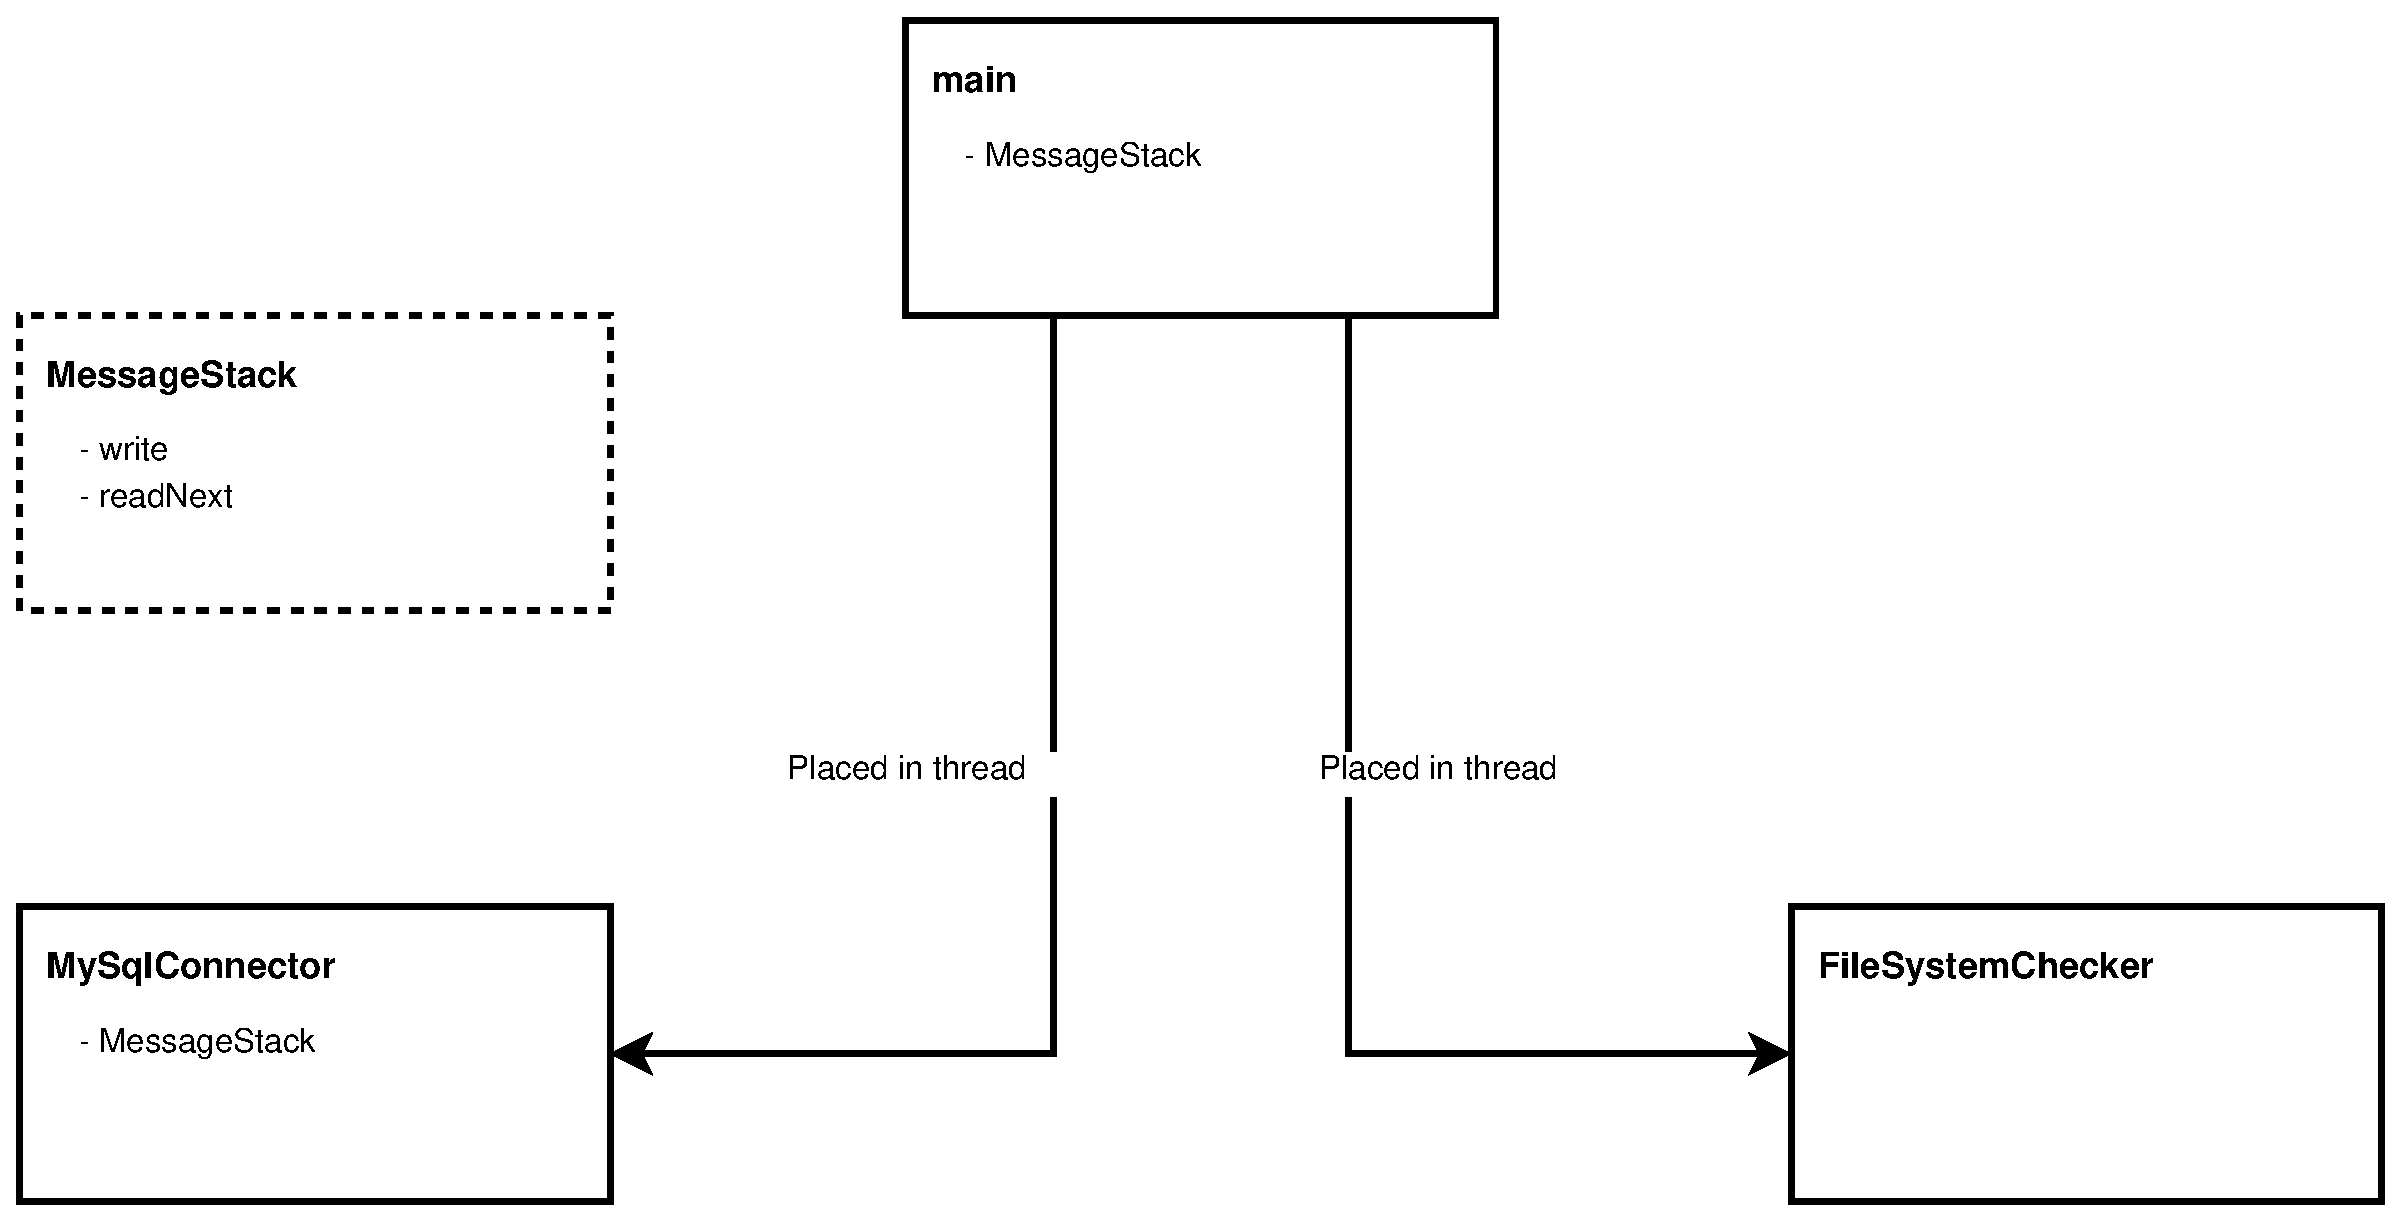
\includegraphics[width=\textwidth]{moose-software-architecture.eps}
    \caption{}
    \label{fig:MOOSE-Arch}
  \end{center}
\end{figure}

The second thread \texttt{main} creates implements a file system checker which continuously scans the directory provided under \texttt{visApiDir} (see Section~\ref{sec:Introduction-Configuration-visApiDir}) for new files. While the content of the files are ignored the file name is used by \ac{MOOSE} to learn about data points it should start or stop receiving by subscribing or unsubscribing for their respective \acp{CID}, respectively.

\section{Data Point Configuration at Run-time}\label{sec:Operations-DataPointConfigAtRuntime}
While \ac{MOOSE} allows users to configure the data points it should subscribe to, a more fine-grained configuration can be achieved at run time via the filesystem. Following the appropriate configuration (see Section~\ref{sec:Introduction-Configuration-visApiDir}) \ac{MOOSE} continuously checks the given folder for new files which indicate the activation or deactivation of data points subscriptions per network entity such as node, port or link. 

If \ac{MOOSE} finds a new file it reads the file name and deletes the file immediately. The syntax of the file name translate into the action \ac{MOOSE} should conduct, i.e.:

\begin{lstlisting}
	NODE_IDENTIFIER-ATTRIBUTE-ACTION
\end{lstlisting}

The \texttt{NODE\_IDENTIFIER} is the unique numerical value representing a particular node in the network and the \texttt{ATTRIBUTE} field the data point \ac{MOOSE} should (de-)activate according to the enumeration \texttt{attribute\_t} in \texttt{apps/monitoring/server/enumerations.hh} or the values in table \texttt{attributes} of the MySQL database. The field \texttt{ACTION} must be either \texttt{enable} or \texttt{disable}.

\end{document}
